\section{Results}

\subsection{Research Question 1: Is Tissue-specific Preference Learnable?}

We first ask whether peptide sequence contains useful tissue-associated signal after holding the MHC restriction and source protein constant. Every retained human or mouse tissue--MHC combination contains more than 200 eligible matched peptide pairs. On the resulting 157-combination human benchmark, the shared-encoder model reaches a mean AUROC of 0.7972 and AUPRC of 0.7829 (Table~\ref{tab:human-standard}), well above random ordering. More structured information sharing increases AUROC to 0.8239--0.8448. Thus, peptides matched by MHC restriction and parent protein are not exchangeable at random, although the observed patterns may reflect antigen processing, protein abundance, cell composition, or study structure.

Human performance after excluding each held-out peptide from all training combinations is reported with the matched ordinary same-pool reference and uncertainty under Research Question 4 (Table~\ref{tab:human-standard-strict-summary}); the identical-fold mouse control comparison is reported under Research Question 7.

\subsection{Research Question 2: Main Human Benchmark Performance}

On the ordinary 157-combination human benchmark, TissuePMHC reaches mean AUROC/AUPRC values of 0.8448/0.8348. Peptides reported in the target tissue generally receive higher scores than their MHC- and parent-protein-matched comparisons, although performance varies markedly across tissue--HLA combinations. Accuracy is 0.7772, MCC is 0.5545, and the mean AUROC of the ten most difficult combinations is 0.6834. Table~\ref{tab:human-standard} compares models on the same combination set.

\begin{table*}[t]
\centering
\caption{Human saved internal test benchmark across 157 tissue--HLA combinations. Mean rows summarize three separately trained models; averaged-model rows are calculated after averaging row-level predictions. Only the two averaged-model rows use directly comparable aggregation.}
\label{tab:human-standard}
\footnotesize
\renewcommand{\arraystretch}{1.20}
\setlength{\tabcolsep}{2pt}
\begin{tabularx}{\textwidth}{>{\raggedright\arraybackslash}Xrrrrrr}
\toprule
Model & \shortstack{Mean\\AUROC} & \shortstack{Median\\AUROC} & AUPRC & Acc. & MCC & Worst-10 \\ 
\midrule
Shared encoder, mean of three runs & 0.7972 & 0.8068 & 0.7829 & 0.7277 & 0.4598 & 0.6299 \\ 
Dual branch with auxiliary supervision, mean of three runs & 0.8239 & 0.8351 & 0.8117 & 0.7552 & 0.5132 & 0.6501 \\ 
Two-view multilayer perceptron, prediction average & 0.8345 & 0.8441 & 0.8233 & 0.7655 & 0.5313 & 0.6666 \\ 
TissuePMHC, prediction average & \textbf{0.8448} & \textbf{0.8585} & \textbf{0.8348} & \textbf{0.7772} & \textbf{0.5545} & \textbf{0.6834} \\ 
\bottomrule
\end{tabularx}
\end{table*}

\begin{figure*}[tbp]
\centering
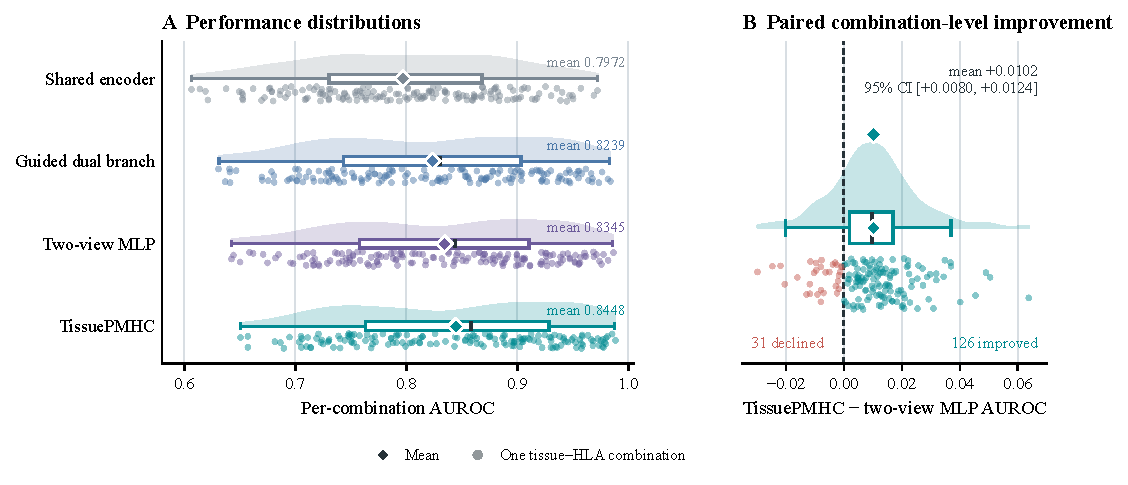
\includegraphics[width=\textwidth]{figures/figure5_human_benchmark_raincloud.pdf}
\caption{Human performance on the ordinary benchmark. \textbf{A}, Raincloud plots show the complete distribution across 157 tissue--HLA combinations: shaded densities summarize distribution shape, points show individual combinations, boxes show the interquartile range and median, and diamonds show the mean. The first two distributions average combination-level AUROCs across three separately trained models; the last two use averaged row-level predictions, matching Table~\ref{tab:human-standard}. \textbf{B}, Paired combination-level AUROC differences between TissuePMHC and the directly comparable two-view multilayer perceptron. The diamond and horizontal interval show the mean difference and its 95\% combination-resampling bootstrap interval (10,000 resamples).}
\label{fig:human-standard}
\end{figure*}

Relative to the directly comparable multilayer perceptron averaged across three runs, TissuePMHC improves mean AUROC by 0.0103 and the difficult-combination summary by 0.0168. The improvement is visible in the mean, median, and lower-performing combinations. Larger differences from the shared-encoder model are descriptive because the aggregation procedures are not identical.

We also repeat the comparison using cross-validation that keeps both rows of every pair in the same fold. This analysis asks whether the advantage extends beyond one saved test set. The closest comparison uses the same two-pathway design with a simpler peptide representation.

\begin{table}[tbp]
\centering
\caption{Human comparison on identical pair-preserving cross-validation folds. This analysis is distinct from the ordinary same-pool reference used to quantify sensitivity to peptide separation.}
\label{tab:human-matched-oof}
\footnotesize
\begin{tabularx}{\columnwidth}{>{\raggedright\arraybackslash}Xrrr}
\toprule
Model & AUROC & AUPRC & Worst-10 \\ 
\midrule
dual-branch model with auxiliary supervision on identical folds & 0.8131 & 0.7980 & 0.6419 \\ 
TissuePMHC & \textbf{0.8279} & \textbf{0.8144} & \textbf{0.6562} \\ 
\bottomrule
\end{tabularx}
\end{table}

The peptide-separated result is reported under Research Question 4 together with its ordinary same-pool reference, a per-combination scatter plot, uncertainty, and four performance measures.

\subsection{Research Question 3: Component Contributions on the Human Benchmark}

Table~\ref{tab:component-evidence} examines whether position-aware filters improve performance, whether global and HLA-specific sharing provide complementary rankings, and whether averaging independent runs improves stability. These are completed system comparisons rather than a full factorial ablation. Replacing the simpler peptide representation with a multi-kernel encoder raises mean AUROC from 0.8345 to 0.8448 and the difficult-combination summary from 0.6666 to 0.6834.

The global pathway performs better on average than the HLA-specific pathway, but their combined within-combination ranking reaches 0.8225--0.8249 AUROC per run, above either pathway alone. Allele-restricted learning therefore contributes useful ordering information for some combinations.

Across three independent runs, TissuePMHC obtains mean AUROCs of 0.8345, 0.8314, and 0.8330, with mean 0.8329 and sample standard deviation 0.0016. Averaging their predictions raises AUROC to 0.8448.

\begin{table*}[t]
\centering
\caption{Evidence about system components from completed runs on the 157-combination human benchmark. The comparisons do not constitute a factorial ablation, and no row isolates a component effect under peptide-separated evaluation.}
\label{tab:component-evidence}
\fontsize{7.5}{8.5}\selectfont
\renewcommand{\arraystretch}{1.20}
\setlength{\tabcolsep}{3pt}
\begin{tabularx}{0.92\textwidth}{@{}>{\raggedright\arraybackslash}p{3.1cm}
                                      >{\raggedright\arraybackslash}X
                                      >{\centering\arraybackslash}p{3.2cm}
                                      >{\centering\arraybackslash}p{1.6cm}@{}}
\toprule
Design question & Completed comparison & AUROC & Descriptive $\Delta$ \\ 
\midrule
Multi-kernel peptide encoding & Multilayer perceptron $\rightarrow$ TissuePMHC; predictions averaged across three runs & 0.8345 $\rightarrow$ 0.8448 & +0.0103 \\ 
Pathway complementarity & Better single pathway $\rightarrow$ combined within-combination ranking; ranges across runs & 0.8072--0.8091 $\rightarrow$ 0.8225--0.8249 & +0.0134--0.0177 \\ 
Prediction averaging & Mean of separate runs $\rightarrow$ average of three prediction sets & 0.8329 $\rightarrow$ 0.8448 & +0.0118 \\ 
\bottomrule
\end{tabularx}
\end{table*}

Together, the ordinary-benchmark runs provide descriptive support for the assembled design but not a causal decomposition of its components. The identical-fold comparisons under Research Question 7 are stronger: auxiliary tissue and allele supervision retains a clear benefit after peptide separation, whereas neither rank fusion without auxiliary supervision nor the multi-kernel encoder shows a stable advantage over the strongest simpler guided model.

\subsection{Research Question 4: Peptides Absent from All Training Combinations}

The ordinary reference repartitions the complete training pair pool. Within each tissue--MHC combination, complete pair identifiers are shuffled using the recorded split random state and assigned round-robin to three folds. This keeps both rows of a pair together but allows a held-out peptide to reappear in fitting rows from another tissue--MHC combination. The peptide-separated analysis starts from the same pair pool but assigns entire groups linked through shared peptide sequences to one fold, ensuring that every held-out peptide is absent from all fitting combinations. Both analyses retain familiar tissue--MHC combinations, evaluate the same pooled rows, and have nearly identical held-out sizes. Their difference measures sensitivity to exact-peptide separation within known biological contexts; it does not test unseen tissues, alleles, combinations, or source proteins.

\subsubsection{Human benchmark}

Removing peptide reuse makes the human ranking problem clearly harder (Table~\ref{tab:human-standard-strict-summary}). Both analyses evaluate the same 73,798 pairs. Among 471 combination-by-fold cells, 333 have identical held-out sizes and the remainder differ by one pair, giving a mean absolute difference of 0.293. In the ordinary folds, 69.19--69.91\% of unique held-out peptides reappear during fitting, compared with 0\% after peptide separation.

\begin{table}[tbp]
\centering
\caption{Human AUROC under same-pool ordinary cross-validation and cross-validation excluding each held-out peptide from all fitting combinations. Difference is peptide-separated minus ordinary same-pool cross-validation; a negative value denotes lower performance after exact peptide separation.}
\label{tab:human-standard-strict-summary}
\footnotesize
\begin{tabularx}{\columnwidth}{>{\raggedright\arraybackslash}X
                            >{\raggedright\arraybackslash}Xr}
\toprule
Ordinary cross-validation & Peptide-separated cross-validation & Difference \\
\midrule
0.8280 & 0.7652 & -0.0628 \\
\bottomrule
\end{tabularx}
\end{table}

Figure~\ref{fig:human-standard-strict-scatter} compares the two AUROC values for each human tissue--HLA combination.
\begin{figure}[!t]
\centering
\begin{tikzpicture}
\begin{groupplot}[
    group style={group size=1 by 1},
    width=0.72\linewidth,
    height=0.52\linewidth,
    xmin=0.5,xmax=1.0,
    ymin=0.5,ymax=1.0,
    xlabel={Ordinary cross-validation AUROC},
    ylabel={Peptide-separated cross-validation AUROC},
    grid=major,
    grid style={gray!20}
]
\nextgroupplot[title={Human tissue--HLA combinations}]
\addplot+[only marks,mark=*,mark size=1.2pt,blue!70] coordinates {(0.96672,0.89632) (0.97035,0.81086) (0.70311,0.67863) (0.80304,0.78235) (0.73140,0.70095) (0.68931,0.62863) (0.77000,0.71465) (0.62590,0.62946) (0.74105,0.70654) (0.75984,0.69934) (0.77139,0.71416) (0.72978,0.72981) (0.75635,0.73227) (0.77172,0.75377) (0.65427,0.63011) (0.71653,0.68030) (0.80139,0.74274) (0.78455,0.76390) (0.77786,0.75187) (0.81349,0.78630) (0.74166,0.76571) (0.82981,0.78587) (0.73312,0.72855) (0.83455,0.83125) (0.85514,0.83040) (0.95176,0.86541) (0.90220,0.70352) (0.92871,0.75592) (0.87940,0.78940) (0.91259,0.87720) (0.88752,0.84003) (0.70758,0.65148) (0.74956,0.74037) (0.77205,0.76026) (0.74550,0.72139) (0.91297,0.87429) (0.91673,0.84768) (0.86843,0.80669) (0.91822,0.86259) (0.92345,0.75413) (0.87903,0.78704) (0.92050,0.80466) (0.86798,0.78964) (0.94395,0.72269) (0.91009,0.75161) (0.85547,0.74550) (0.82809,0.64234) (0.96895,0.89676) (0.91098,0.71989) (0.87057,0.80826) (0.93357,0.81315) (0.94807,0.77722) (0.82663,0.72979) (0.91800,0.83660) (0.95452,0.87204) (0.84433,0.80015) (0.92370,0.83370) (0.96999,0.80102) (0.78527,0.66459) (0.87280,0.84343) (0.88053,0.80683) (0.66490,0.65294) (0.77697,0.66023) (0.86138,0.78989) (0.90441,0.79441) (0.77384,0.75616) (0.90932,0.74419) (0.76607,0.74991) (0.84100,0.82669) (0.72223,0.69249) (0.85461,0.78063) (0.81206,0.65929) (0.72648,0.73876) (0.63959,0.61426) (0.80413,0.80050) (0.69950,0.74672) (0.78296,0.73935) (0.70276,0.70267) (0.87707,0.86354) (0.91622,0.79570) (0.96027,0.79787) (0.80585,0.78590) (0.77018,0.76059) (0.81372,0.79084) (0.88963,0.86683) (0.87950,0.83954) (0.87368,0.83389) (0.75885,0.75382) (0.65223,0.61726) (0.83946,0.77236) (0.65179,0.67576) (0.84010,0.82535) (0.78485,0.75757) (0.74455,0.71806) (0.74341,0.70407) (0.76307,0.71106) (0.80130,0.79016) (0.86440,0.84891) (0.67262,0.75955) (0.77538,0.77245) (0.82222,0.87481) (0.76653,0.73348) (0.72877,0.71012) (0.76004,0.74685) (0.75181,0.70336) (0.83289,0.77030) (0.78132,0.76907) (0.74148,0.74364) (0.64481,0.67523) (0.85471,0.85110) (0.84419,0.82932) (0.76748,0.75360) (0.66622,0.72145) (0.76186,0.73488) (0.75690,0.74757) (0.89072,0.88061) (0.82900,0.81400) (0.72541,0.67367) (0.83158,0.83090) (0.91507,0.86390) (0.84504,0.71075) (0.98888,0.78529) (0.81338,0.76173) (0.94582,0.71469) (0.92700,0.81194) (0.93426,0.74075) (0.95187,0.87273) (0.87999,0.73061) (0.91318,0.83304) (0.75517,0.72200) (0.80923,0.65597) (0.86547,0.72009) (0.91214,0.86378) (0.94262,0.87700) (0.87746,0.81565) (0.75234,0.70200) (0.89621,0.81584) (0.83017,0.76067) (0.84406,0.71097) (0.75516,0.68902) (0.94164,0.71440) (0.90257,0.77277) (0.93696,0.76132) (0.83397,0.71052) (0.93787,0.77398) (0.95530,0.78414) (0.94340,0.86661) (0.82934,0.79463) (0.84995,0.82641) (0.72547,0.72614) (0.82860,0.81765) (0.75124,0.72947) (0.80609,0.75079) (0.74374,0.69960) (0.97196,0.89320) (0.92317,0.73906) (0.95193,0.79084)};
\addplot+[black!65,densely dashed,very thick,no marks,domain=0.5:1.0] {x};
\end{groupplot}
\end{tikzpicture}
\caption{Human AUROC for each tissue--HLA combination under ordinary same-pool and peptide-separated cross-validation. Points below the gray equality line have lower performance after exact-peptide separation.}
\label{fig:human-standard-strict-scatter}
\end{figure}

Mean human AUROC decreases by 0.0628 and is lower for 145 of 157 tissue--HLA combinations. The 95\% interval obtained by resampling complete combinations is -0.0728 to -0.0534. Within-pair ordering accuracy decreases by 0.0529. Exact peptide reuse therefore explains part, but not all, of the easier performance estimate.

\subsubsection{Mouse benchmark}

The mouse peptide-separated benchmark uses the same 6,766 pairs, grouped into 1,844 peptide-linked components with zero held-out-peptide overlap. A matched ordinary-versus-separated estimate is not reported here because the retained mouse controls were not all evaluated under a common ordinary-fold protocol. Their identical-fold peptide-separated comparison is reported under Research Question 7.

Saved-test results are not subtracted from peptide-separated cross-validation results because the evaluations contain different examples.

The peptide-separated analysis removes exact-peptide reuse while retaining familiar tissue--MHC combinations and other shared context. Table~\ref{tab:evaluation-protocols} and the Limitations define its scope.

\subsection{Research Question 5: Replication in Mouse Tissue--MHC (H-2) Combinations}

The mouse benchmark asks whether the same MHC- and parent-protein-controlled comparison is learnable across 24 tissue--H2 combinations. Mouse models are trained independently, and no human parameters are transferred.

\begin{table*}[t]
\centering
\caption{Expanded retrospective method survey on the mouse saved internal test set across 24 tissue--H2 combinations. Ordinary rows are arithmetic means of three runs (seeds 20260704--20260706); rows marked $\dagger$ aggregate row-level predictions across the stated runs. Worst-6 is the mean AUROC of the six lowest-performing combinations within each run or prediction aggregate.}
\label{tab:mouse-baselines}
\footnotesize
\renewcommand{\arraystretch}{1.06}
\setlength{\tabcolsep}{2.5pt}
\begin{tabularx}{\textwidth}{>{\raggedright\arraybackslash}Xrrr
                            >{\raggedright\arraybackslash}p{2.5cm}}
\toprule
Model & AUROC & AUPRC & Worst-6 & Evidence \\ 
\midrule
Neural single-task MLP & 0.7315 & 0.7078 & 0.6424 & three-run mean \\
Tissue-grouped hard sharing & 0.7329 & 0.7104 & 0.6460 & three-run mean \\
Conditioned tissue and H2 IDs & 0.8158 & 0.8118 & 0.6689 & three-run mean \\
Selective global/H2 grouping & 0.8258 & 0.8192 & 0.6907 & three-run mean \\
DB-MTL shared heads & 0.8301 & 0.8207 & 0.6942 & three-run mean \\
MMoE, 4 experts $\times$ width 256 & 0.8309 & 0.8227 & 0.6963 & three-run mean \\
MMoE, 6 experts $\times$ width 128 & 0.8315 & 0.8268 & 0.7023 & three-run mean \\
Validation-softmax dual-branch ensemble & 0.8329 & 0.8275 & 0.6965 & three-run mean \\
Shared encoder with task heads & 0.8333 & 0.8254 & 0.6965 & three-run mean \\
Validation-delta clipped dual-branch ensemble & 0.8355 & 0.8295 & 0.7005 & three-run mean \\
Fixed global/H2 dual-branch average & 0.8372 & 0.8304 & 0.7031 & three-run mean \\
Auxiliary-global + auxiliary-H2 dual branch & 0.8400 & 0.8340 & 0.7057 & three-run mean \\
Auxiliary-global + plain-H2 dual branch & 0.8415 & 0.8356 & 0.7068 & three-run mean \\
MLP dual-branch rank average$^\dagger$ & 0.8488 & 0.8436 & 0.7153 & three-run aggregate \\
Full multi-kernel TissuePMHC$^\dagger$ & \textbf{0.8528} & \textbf{0.8477} & \textbf{0.7196} & three-run aggregate \\
\bottomrule
\end{tabularx}
\end{table*}

Table~\ref{tab:mouse-baselines} adds the completed mouse implementations of method families evaluated in the human benchmark. Every row uses the same fixed mouse training and test partitions, and every metric gives equal weight to the 24 combinations. The H2 pseudo-sequence-conditioned and ID--pseudo-sequence hybrid models are omitted because no provenance-verified H2 pseudo-sequence file was available. The full multi-kernel TissuePMHC aggregate is numerically strongest, followed by the MLP dual-branch aggregate. Because multiple architectures have been compared retrospectively on the saved test set, this survey is an internal benchmark comparison rather than untouched confirmation or external validation.

\begin{table*}[!t]
\centering
\caption{Mouse saved-test AUROC grouped by H2 restriction. Values are descriptive subgroup means rather than controlled restriction effects.}
\label{tab:mouse-h2-groups}
\small
\begin{tabularx}{\textwidth}{>{\raggedright\arraybackslash}X
                            >{\centering\arraybackslash}X
                            >{\centering\arraybackslash}X
                            >{\centering\arraybackslash}X
                            >{\centering\arraybackslash}X}
\toprule
H2 restriction & H2-Db & H2-Kb & H2-Kd & H2-Kk \\ 
\midrule
Mean AUROC across tissues & 0.9152 & 0.7404 & 0.8397 & 0.8024 \\ 
\bottomrule
\end{tabularx}
\end{table*}

On the saved internal test set, the strongest retained prediction aggregate has an equal-weight AUROC/AUPRC of 0.8528/0.8477. Because the same saved benchmark was used for the retrospective method survey, this value characterizes the observed benchmark rather than providing independent validation. Peptide-separated results for the matched mouse controls are reported under Research Question 7.

\subsection{Research Question 6: How Much Signal Remains without Tissue Identity?}

Removing tissue identity while retaining peptide and MHC information lowers human performance in every evaluation. Under peptide-separated cross-validation, AUROC falls from 0.7652 to 0.6630, with decreases in 156 of 157 combinations. General peptide--MHC compatibility therefore does not reproduce the complete ranking signal, although this does not prove a causal tissue-processing mechanism.

This comparison must be interpreted together with the conflict audit in Table~\ref{tab:tissue-blind-conflict-audit}. Once tissue is hidden, an identical peptide--MHC input can retain different labels from different tissue contexts. The performance decrease therefore reflects the information lost with tissue identity, including the resulting input--label ambiguity; it should not be attributed solely to a molecular tissue-processing effect.

\begin{table*}[t]
\centering
\caption{Human comparison of controls that omit tissue identity with the full tissue-conditioned TissuePMHC model. The control retaining peptide and MHC information has approximately the same capacity as the full model. MHCflurry uses its predicted-presentation score and NetMHCpan its eluted-ligand score. External scores are predetermined, so their values are identical across the two cross-validation partitions of the same pool.}
\label{tab:rq6-method-comparison}
\footnotesize
\renewcommand{\arraystretch}{0.9}
\setlength{\tabcolsep}{2pt}
\begin{tabular}{@{}>{\raggedright\arraybackslash}p{4.4cm}
                   >{\centering\arraybackslash}p{2.2cm}
                   >{\centering\arraybackslash}p{2.2cm}
                   >{\centering\arraybackslash}p{2.2cm}
                   >{\bfseries\centering\arraybackslash}p{2.2cm}@{}}
\toprule
Evaluation metric & Peptide + MHC & \shortstack{MHCflurry\\presentation} & \shortstack{NetMHCpan\\eluted-ligand score} & \shortstack{\textbf{Full}\\\textbf{tissue-conditioned}} \\
\midrule
\multicolumn{5}{@{}l}{\textit{Human}} \\
Saved internal test: AUROC & 0.7449 & 0.6851 & 0.6833 & 0.8448 \\
Saved internal test: AUPRC & 0.7563 & 0.6783 & 0.6686 & 0.8348 \\
Saved internal test: within-pair accuracy & 0.7243 & 0.6886 & 0.6897 & 0.8375 \\
\addlinespace
Same-pool ordinary cross-validation: AUROC & 0.7353 & 0.6871 & 0.6823 & 0.8279 \\
Same-pool ordinary cross-validation: AUPRC & 0.7379 & 0.6751 & 0.6632 & 0.8144 \\
Same-pool ordinary cross-validation: within-pair accuracy & 0.7144 & 0.6898 & 0.6875 & 0.8229 \\
\addlinespace
Peptide-separated cross-validation: AUROC & 0.6630 & 0.6871 & 0.6823 & 0.7652 \\
Peptide-separated cross-validation: AUPRC & 0.6502 & 0.6751 & 0.6632 & 0.7452 \\
Peptide-separated cross-validation: within-pair accuracy & 0.6691 & 0.6898 & 0.6875 & 0.7700 \\
\bottomrule
\end{tabular}
\end{table*}

MHCflurry and NetMHCpan perform better than random on the human matched pairs (Table~\ref{tab:rq6-method-comparison}). General binding and presentation propensity therefore contribute useful information. The full tissue-conditioned model nevertheless has the highest value for every reported metric and evaluation.

The NetMHCpan eluted-ligand score is consistently at least as strong as its binding-affinity score. The AUROC difference between eluted-ligand score and binding-affinity score is 0.0256 on the human saved internal test set and 0.0264 on the human complete training pool. We therefore use the eluted-ligand score as the primary NetMHCpan control and report the complete binding-affinity score sensitivity analysis in Table~\ref{tab:appendix-netmhcpan-el-ba}.

The human tissue-conditioned model remains higher than the strongest tissue-agnostic control in every evaluation. AUROC is 0.8448 versus 0.6851 on the saved test, 0.8279 versus 0.6871 under ordinary same-pool cross-validation, and 0.7652 versus 0.6871 after peptide separation; the peptide-separated advantage is 0.0781.

Cross-fitted stacking yields only marginal improvement over the human tissue-conditioned score alone. The largest change is observed for peptide-separated cross-validation with MHCflurry, from 0.7652 to 0.7693 AUROC; the saved-test value changes from 0.8448 to 0.8453. Complete results appear in Table~\ref{tab:appendix-general-stacking}.

\subsection{Research Question 7: Model Structure under Peptide Separation}

Every model is retrained on the same peptide-separated folds. All human models retain useful signal (Table~\ref{tab:human-strict-architectures}). TissuePMHC clearly exceeds simple sequence baselines and modestly exceeds the shared encoder and unguided dual-branch models.

\begin{table*}[t]
\centering
\caption{Human architecture comparison across 157 tissue--HLA combinations on identical peptide-separated folds. Neural methods average row-level predictions across runs; logistic regression has no random training variation.}
\label{tab:human-strict-architectures}
\fontsize{7.5}{8.5}\selectfont
\renewcommand{\arraystretch}{0.98}
\setlength{\tabcolsep}{2pt}
\begin{tabularx}{\textwidth}{>{\raggedright\arraybackslash}Xrrrrrr}
\toprule
Model & Mean AUROC & Median & AUPRC & \shortstack{Within-pair\\accuracy} & Worst-10 & Worst combination \\
\midrule
One-hot logistic regression & 0.7127 & 0.7069 & 0.6906 & 0.7157 & 0.5873 & 0.5533 \\
BLOSUM62 random forest & 0.7212 & 0.7208 & 0.7007 & 0.7263 & 0.5895 & 0.5634 \\
Shared encoder & 0.7561 & 0.7565 & 0.7340 & 0.7631 & 0.6248 & 0.6003 \\
Dual branch without auxiliary supervision & 0.7555 & 0.7577 & 0.7339 & 0.7575 & 0.6163 & 0.5905 \\
Dual branch with auxiliary supervision & 0.7642 & \textbf{0.7660} & 0.7433 & 0.7686 & 0.6283 & 0.6034 \\
TissuePMHC & \textbf{0.7652} & 0.7606 & \textbf{0.7452} & \textbf{0.7700} & \textbf{0.6382} & \textbf{0.6142} \\
\bottomrule
\end{tabularx}
\end{table*}

\begin{table*}[t]
\ContinuedFloat
\centering
\caption[]{Human architecture comparison (continued): retrospective survey on the saved internal test set. These rows use the 157 tissue--HLA combinations in the saved-test benchmark and are not directly comparable to the peptide-separated rows in the preceding panel. Ordinary neural rows are arithmetic means of three runs; rows marked $\dagger$ aggregate row-level predictions.}
\fontsize{7.5}{8.5}\selectfont
\renewcommand{\arraystretch}{0.98}
\setlength{\tabcolsep}{2pt}
\begin{tabularx}{\textwidth}{>{\raggedright\arraybackslash}Xrrrrr
                            >{\raggedright\arraybackslash}p{1.7cm}}
\toprule
Model & AUROC & AUPRC & Acc. & MCC & Worst-10 & Evidence \\
\midrule
One-hot logistic regression & 0.7238 & 0.7065 & 0.6636 & 0.3288 & 0.5939 & single fit \\
BLOSUM62 logistic regression & 0.7227 & 0.6985 & 0.6672 & 0.3357 & 0.5950 & single fit \\
BLOSUM62 HistGradientBoosting & 0.7240 & 0.7066 & 0.6668 & 0.3351 & 0.5893 & single fit \\
BLOSUM62 Extra Trees & 0.7279 & 0.7120 & 0.6680 & 0.3386 & 0.5958 & single fit \\
BLOSUM62 random forest & 0.7297 & 0.7146 & 0.6707 & 0.3444 & 0.5969 & single fit \\
Neural single-task MLP & 0.6934 & 0.6803 & 0.6410 & 0.2841 & 0.5682 & three-run mean \\
Shared encoder with task heads & 0.7972 & 0.7829 & 0.7277 & 0.4598 & 0.6299 & three-run mean \\
Conditioned tissue and HLA IDs & 0.7955 & 0.7856 & 0.7309 & 0.4648 & 0.5662 & three-run mean \\
HLA pseudo-sequence conditioned & 0.7866 & 0.7761 & 0.7258 & 0.4549 & 0.5371 & three-run mean \\
HLA ID + pseudo-sequence hybrid & 0.7963 & 0.7867 & 0.7334 & 0.4701 & 0.5667 & three-run mean \\
FAMO shared heads & 0.7668 & 0.7518 & 0.7038 & 0.4103 & 0.5997 & three-run mean \\
HLA-grouped hard sharing & 0.7972 & 0.7855 & 0.7347 & 0.4716 & 0.5942 & three-run mean \\
Tissue-grouped hard sharing & 0.7122 & 0.6946 & 0.6549 & 0.3122 & 0.5878 & three-run mean \\
Selective global/HLA grouping & 0.8035 & 0.7902 & 0.7377 & 0.4788 & 0.6137 & three-run mean \\
Fixed global/HLA dual-branch average & 0.8184 & 0.8069 & 0.7513 & 0.5055 & 0.6440 & three-run mean \\
Validation-delta clipped ensemble & 0.8175 & 0.8061 & 0.7495 & 0.5019 & 0.6354 & three-run mean \\
Validation-softmax ensemble & 0.8136 & 0.8020 & 0.7458 & 0.4947 & 0.6259 & three-run mean \\
MMoE & 0.8070 & 0.7930 & 0.7381 & 0.4822 & 0.6379 & three-run mean \\
MMoE, 4 experts $\times$ width 256 & 0.8076 & 0.7945 & 0.7388 & 0.4833 & 0.6271 & three-run mean \\
MMoE, 6 experts $\times$ width 128 & 0.8050 & 0.7920 & 0.7356 & 0.4759 & 0.6319 & three-run mean \\
DB-MTL shared heads & 0.7820 & 0.7672 & 0.7172 & 0.4369 & 0.5972 & three-run mean \\
Pair-ranking objective & 0.7849 & 0.7692 & 0.7209 & 0.4438 & 0.6059 & three-run mean \\
Tissue/HLA auxiliary supervision & 0.8082 & 0.7921 & 0.7353 & 0.4772 & 0.6474 & three-run mean \\
Auxiliary-global + plain-HLA dual branch & 0.8239 & 0.8117 & 0.7552 & 0.5132 & 0.6501 & three-run mean \\
Auxiliary-global + auxiliary-HLA dual branch & 0.8202 & 0.8082 & 0.7510 & 0.5056 & 0.6502 & three-run mean \\
MLP dual-branch rank average$^\dagger$ & 0.8345 & 0.8233 & 0.7655 & 0.5313 & 0.6666 & three-run aggregate \\
Full multi-kernel TissuePMHC$^\dagger$ & \textbf{0.8448} & \textbf{0.8348} & \textbf{0.7772} & \textbf{0.5545} & \textbf{0.6834} & three-run aggregate \\
\bottomrule
\end{tabularx}
\end{table*}

The saved-test continuation broadens the retrospective survey without changing the protocol-specific conclusions. The full TissuePMHC prediction aggregate is numerically strongest, followed by the MLP dual-branch aggregate. Among ordinary three-run means, the auxiliary-global plus plain-HLA dual branch is strongest. These comparisons reuse the saved benchmark and therefore support method characterization rather than independent model selection.

\begin{table*}[!b]
\centering
\caption{Mouse architecture comparison across 24 tissue--H2 combinations on identical peptide-separated folds. All entries average predictions across five runs.}
\label{tab:mouse-strict-architectures}
\fontsize{7.5}{8.5}\selectfont
\renewcommand{\arraystretch}{0.98}
\setlength{\tabcolsep}{1pt}
\begin{tabularx}{\textwidth}{>{\raggedright\arraybackslash}Xrrrrrr}
\toprule
Model & Mean AUROC & Median & AUPRC & \shortstack{Within-pair\\accuracy} & Worst-6 & Worst combination \\
\midrule
One-hot logistic regression & 0.7335 & 0.7395 & 0.7050 & 0.7363 & 0.6266 & 0.5709 \\
BLOSUM62 random forest & 0.7507 & 0.7768 & 0.7295 & 0.7573 & 0.6418 & \textbf{0.5819} \\
Shared encoder & 0.7538 & 0.7786 & 0.7321 & 0.7567 & 0.6430 & 0.5477 \\
Dual branch without auxiliary supervision & 0.7556 & 0.7758 & 0.7372 & 0.7542 & 0.6416 & 0.5496 \\
Dual branch with auxiliary supervision & \textbf{0.7590} & \textbf{0.7797} & \textbf{0.7395} & \textbf{0.7605} & \textbf{0.6464} & 0.5494 \\
\bottomrule
\end{tabularx}
\end{table*}

\begin{figure*}[t]
\centering
\begin{tikzpicture}
\begin{groupplot}[
    group style={group size=1 by 2,vertical sep=0.95cm},
    width=0.97\textwidth,
    height=4.25cm,
    xmin=0.6,xmax=15.4,
    ymin=0.66,ymax=0.86,
    xtick={1,...,15},
    ytick={0.68,0.72,0.76,0.80,0.84},
    ylabel={Score},
    grid=major,
    grid style={gray!20},
    tick align=outside,
    every axis plot/.append style={line width=0.8pt,mark size=2pt},
    legend style={draw=none,fill=none,font=\small,
                  at={(0.99,0.03)},anchor=south east,
                  legend columns=2},
    legend cell align=left
]
\nextgroupplot[
    title={AUROC},
    xticklabels={}
]
\addplot[color=blue!75!black,mark=*,solid]
coordinates {(1,0.6934) (2,0.7972) (3,0.7955) (4,0.7122) (5,0.8035)
             (6,0.8184) (7,0.8175) (8,0.8136) (9,0.8076) (10,0.8050)
             (11,0.7820) (12,0.8239) (13,0.8202) (14,0.8345) (15,0.8448)};
\addlegendentry{Human}
\addplot[color=orange!85!black,mark=square*,dashed]
coordinates {(1,0.7315) (2,0.8333) (3,0.8158) (4,0.7329) (5,0.8258)
             (6,0.8372) (7,0.8355) (8,0.8329) (9,0.8309) (10,0.8315)
             (11,0.8301) (12,0.8415) (13,0.8400) (14,0.8488) (15,0.8528)};
\addlegendentry{Mouse}

\nextgroupplot[
    title={AUPRC},
    xticklabels={ST-MLP,Shared,Cond-ID,Tissue-HS,Sel-G/MHC,Fixed-DB,
                 $\Delta$-ens.,Softmax-ens.,MMoE-4,MMoE-6,DB-MTL,
                 AuxG+plain,AuxG+aux,DB-rank,TissuePMHC},
    x tick label style={rotate=48,anchor=east,font=\scriptsize},
    xlabel={Algorithm family in experimental order},
    xlabel style={yshift=-0.15cm}
]
\addplot[color=blue!75!black,mark=*,solid]
coordinates {(1,0.6803) (2,0.7829) (3,0.7856) (4,0.6946) (5,0.7902)
             (6,0.8069) (7,0.8061) (8,0.8020) (9,0.7945) (10,0.7920)
             (11,0.7672) (12,0.8117) (13,0.8082) (14,0.8233) (15,0.8348)};
\addplot[color=orange!85!black,mark=square*,dashed]
coordinates {(1,0.7078) (2,0.8254) (3,0.8118) (4,0.7104) (5,0.8192)
             (6,0.8304) (7,0.8295) (8,0.8275) (9,0.8227) (10,0.8268)
             (11,0.8207) (12,0.8356) (13,0.8340) (14,0.8436) (15,0.8477)};
\end{groupplot}
\end{tikzpicture}
\caption{Score trends for matched algorithm families evaluated separately on the human and mouse saved internal test benchmarks. The upper and lower panels show AUROC and AUPRC, respectively. Algorithm families follow the experimental order used in the original comparison; connecting lines guide cross-species trend comparison and do not imply a continuous optimization trajectory. Ordinary points are three-run means, whereas DB-rank and TissuePMHC aggregate row-level predictions across three runs. ST-MLP denotes the neural single-task MLP; Cond-ID, conditioned tissue and MHC IDs; Tissue-HS, tissue-grouped hard sharing; Sel-G/MHC, selective global/MHC grouping; DB, dual branch; ens., ensemble; and AuxG, auxiliary-global. Each species uses its own training data, task inventory, and MHC representation, so the gaps are not estimates of a species effect.}
\label{fig:cross-species-same-algorithms}
\end{figure*}

Across the 15 shared algorithm families in Figure~\ref{fig:cross-species-same-algorithms}, the mouse saved-test AUROC is numerically higher by 0.0080--0.0481. The ordering is nevertheless broadly consistent: dual-branch prediction aggregates occupy the strongest end in both species, whereas single-task and tissue-grouped training are weaker. Dataset size, task composition, allele inventory, and test examples differ, so the numerical gaps cannot be attributed to species.

Comparison with the strongest simpler human control warrants caution. The guided dual-branch model uses the same two-pathway structure with a simpler peptide representation. TissuePMHC is only 0.0010 AUROC higher, with 76 positive, one tied, and 80 negative per-combination differences; the uncertainty interval includes zero. By contrast, adding tissue and HLA supervision to the unguided dual branch improves AUROC by 0.0087 and benefits 144 of 157 combinations. The clearest retained effect is therefore biological-group supervision rather than the more elaborate encoder alone.

The mouse comparison matches the human strict table for one-hot logistic regression, BLOSUM62 random forest, shared encoding, and the two dual-branch controls (Table~\ref{tab:mouse-strict-architectures}). The auxiliary dual branch has the highest mean AUROC (0.7590). Auxiliary supervision improves the matched dual branch by 0.0034 AUROC and is higher in 21 of 24 combinations (95\% interval, 0.0023--0.0047). Mean AUROC differs by at most 0.0083 among the random forest, shared encoder, and two dual-branch models. Thus, peptide-separated mouse performance supports learnability and a small benefit from auxiliary supervision rather than broad architectural superiority.

Prediction averaging materially improves the final neural estimates. Relative to the mean of separate runs, AUROC gains are +0.0248 for the human shared encoder, +0.0161 for the unguided dual branch, +0.0139 for the guided dual branch, and +0.0147 for TissuePMHC\@. Mouse gains are +0.0211 for the shared encoder, +0.0175 for the unguided dual branch, and +0.0167 for the auxiliary dual branch, compared with +0.0016 for the random forest and zero for one-hot logistic regression.
